

  In the right triangle below, what is $\tan(x)$?
 \begin{center}
 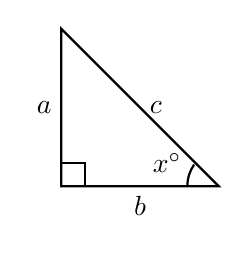
\begin{tikzpicture}
 
 \draw (0,0) --(2,0)--(0,2)--cycle  [thick,-,>=latex];
 \draw (0,0) --(0,.3)--(.3,.3)--(.3,0)--cycle  [thick,-,>=latex];
\draw[thick] (1.6,0) arc (180:145:.48);

  \draw node[left] at (1.65,.3) {$x^\circ$};
  \draw node[left] at (0,1) {$a$};
   \draw node[below] at (1,0) {$b$};
   \draw node[right] at (1,1) {$c$};

\end{tikzpicture}
\end{center}




\ifsat
	\begin{enumerate}[label=\Alph*)]
		\item    $\frac{a}{b}$ %
		\item  $\frac{b}{a}$ 
		\item $\frac{a}{\sqrt{a^{2}+b^{2}}}$ 
		\item $\frac{b}{\sqrt{a^{2}+b^{2}}}$ 
	\end{enumerate}
\else
\fi

\ifacteven
	\begin{enumerate}[label=\textbf{\Alph*.},itemsep=\fill,align=left]
		\setcounter{enumii}{5}
		\item    $\frac{a}{b}$ %
		\item  $\frac{b}{a}$ 
		\item $\frac{a}{\sqrt{a^{2}+b^{2}}}$ 
		\addtocounter{enumii}{1}
		\item $\frac{b}{\sqrt{a^{2}+b^{2}}}$ 
		\item  Cannot be determined
	\end{enumerate}
\else
\fi

\ifactodd
	\begin{enumerate}[label=\textbf{\Alph*.},itemsep=\fill,align=left]
		\item    $\frac{a}{b}$ %
		\item  $\frac{b}{a}$ 
		\item $\frac{a}{\sqrt{a^{2}+b^{2}}}$ 
		\item $\frac{b}{\sqrt{a^{2}+b^{2}}}$ 
		\item  Cannot be determined
	\end{enumerate}
\else
\fi

\ifgridin
    $\frac{a}{b}$ %
		
\else
\fi

